\begin{figure*}[tb]
  \centering
  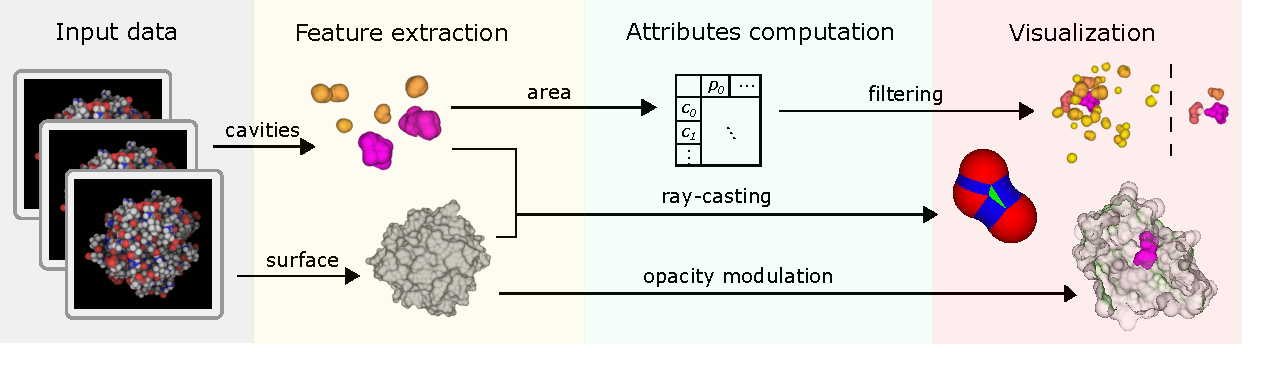
\includegraphics[width=\textwidth]{image/overview.pdf}
  \caption{Illustration of the visualization pipeline. The input data contains snapshots of MD trajectories which are processed to construct the molecular surface elements and cavities. Further, the surface areas of cavities are estimated, which are used as the color codes, ranging from yellow (smallest) to red (largest). Finally, the surface elements are ray-casted to compose the surface fragments used in the final stage to visualize the surfaces transparently via a user defined opacity modulation.}
	\label{fig:overview}
\end{figure*}

The computation of SES is not a trivial task that requires substantial computation and algorithmic capabilities. 
Therefore, it would be essential to posses a technique that could provide us with an instant computation, and interactive and meaningful visualization of cavities in the context of molecular surface.

The data comes in a form of MD trajectories describing the motion of individual atoms. 
Each trajectory snapshot includes a set of atoms, described by their positions and their radii. 
Our rendering pipeline consists of several steps that are performed on a per-frame basis. 
For better explanation, we split the computations into two groups. 
The first group deals with data processing that involves the computation of the surface primitives, and inner voids, i.e., cavities.
The second group of computations relates to visualization. 
This group includes estimating sizes of voids, ray-casting of the generated surface primitives and opacity calculation; before the final stage represented by the image formation. More specifically, we perform the following steps (Fig.~\ref{fig:overview}):
	\begin{enumerate}
	  \item We employ the contour-buildup algorithm to construct the molecular surface. Additionally, we enhance the computation to enable i) transparent rendering of the surface and ii) extraction of cavities (Sec.~\ref{sec:ecb}).
		\item For cavity extraction, we introduce the so-called \textit{surface graph} (Sec.~\ref{sec:graph}), which allows us to detect isolated surface components.
		\item We estimate area of the extracted cavities to enable a color coding by their size and to lower potential clutter by hiding small cavities.
		\item Surface elements are visualized using ray-casting (Sec.~\ref{sec:vis}). We perform transparent surface rendering by means of an A-buffer and an opacity modulation. The modulation is based on an estimate of the molecular thickness per each surface fragment on the given ray and a set of user defined parameters.
	\end{enumerate}